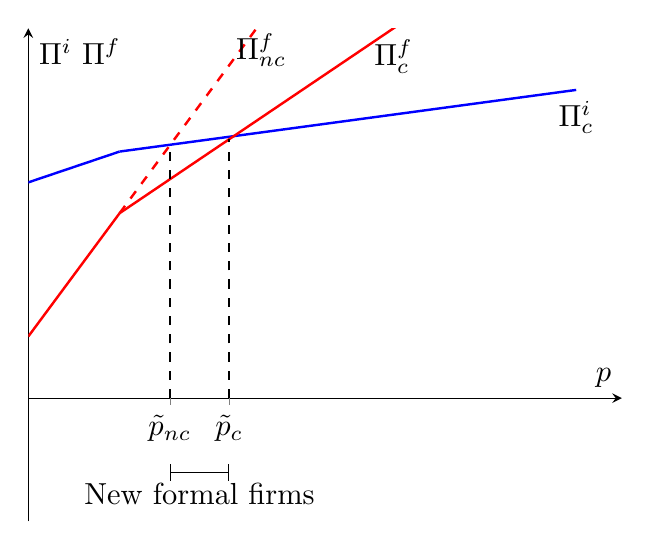
\begin{tikzpicture}[scale=1.1, transform shape]
\begin{axis}[
    axis lines=middle,
    xlabel=$p$,
    ylabel=$\Pi^i$ $\Pi^f$,
    xmin=0,
    ymin=-2,
    xmax=6.5,
    ymax=6,
    legend pos=outer north east,
    grid=none,
    xtick=\empty,  % Remove x-axis tick labels and ticks
    ytick=\empty,  % Remove y-axis tick labels and ticks
    extra x ticks={1.55, 2.2},
    extra x tick labels={$\tilde{p}_{nc}$, $\tilde{p}_{c}$},
]

% Plot the initial portion (y=0)
\addplot[domain=0:1, blue, thick, samples=100] {(1/2)*x+3.5};

% \addplot[domain=1:6, blue, thick, dashed, samples=100] {(1/2)*x+3.5} node[pos=1, below, black] {$\Pi^i$};

\addplot[domain=1:6, blue, thick, samples=100] {(1/5)*x+3.8} node[pos=1, below, black] {$\Pi^i_{c}$};



% Plot the transition
\addplot[domain=0:1, red, thick, samples=100] {2*x+1};

\addplot[domain=1:6, red, thick, dashed, samples=100] {2*x+1} node[pos=0.31, below, black] {$\Pi^f_{nc}$};

\addplot[domain=1:6, red, thick, samples=100] {1*x+2} node[pos=0.6, below, black] {$\Pi^f_{c}$};

% Add a vertical dashed line at x=3
\draw[dashed, black, thick] (axis cs:2.2,0) -- (axis cs:2.2,4.2);

\draw[dashed, black, thick] (axis cs:1.55,0) -- (axis cs:1.55,4.1);


\draw[|-|] (axis cs:1.55,-1.2) -- node[below] {New formal firms} (axis cs:2.2,-1.2);



\end{axis}
\end{tikzpicture}

24
